% (c) 2001-2011 Ben Crowell, licensed under the Creative Commons
% Attribution-ShareAlike license,
% http://creativecommons.org/licenses/by-sa/1.0/
%
\documentclass{lmseries}
% \let\ifpdf\relax % http://tex.stackexchange.com/questions/11414/package-ifpdf-error
% --------> this fails with TeX Live 2013, conflicts with xparse
%\selectlanguage{english}
\usepackage{lmlanguage}
%\includeonly{n1/ctemp}
\inputprotcode
\makeindex
\pdfmapfile{=fullembed.map} % created by the script create_fullembed_file
\begin{document}
\myeqnspacing % Do this early and often, since it gets reset by \normalsize
% 
% The following is all related to margin kerning.
% This is activated in dp.cls using the boolean wantmarginkerning.
% The constant 1 is to allow margin kerning, but to keep it from affecting
% line breaks.
\ifthenelse{\boolean{wantmarginkerning}}{
 \setprotcode\font
 {\it \setprotcode \font}
 {\bf \setprotcode \font}
 {\bf \it \setprotcode \font}
 \pdfprotrudechars=1
}{}
%========================= frontmatter =========================
\formatchtoc{\Large}{}{4mm}
\frontmatter
\yesiwantarabic
\renewcommand{\chapdir}{front}
\thispagestyle{empty}
\raisebox{0mm}[0mm][0mm]{%
\parbox{8.5in}{
\vspace*{236mm}\hspace{-38.5mm}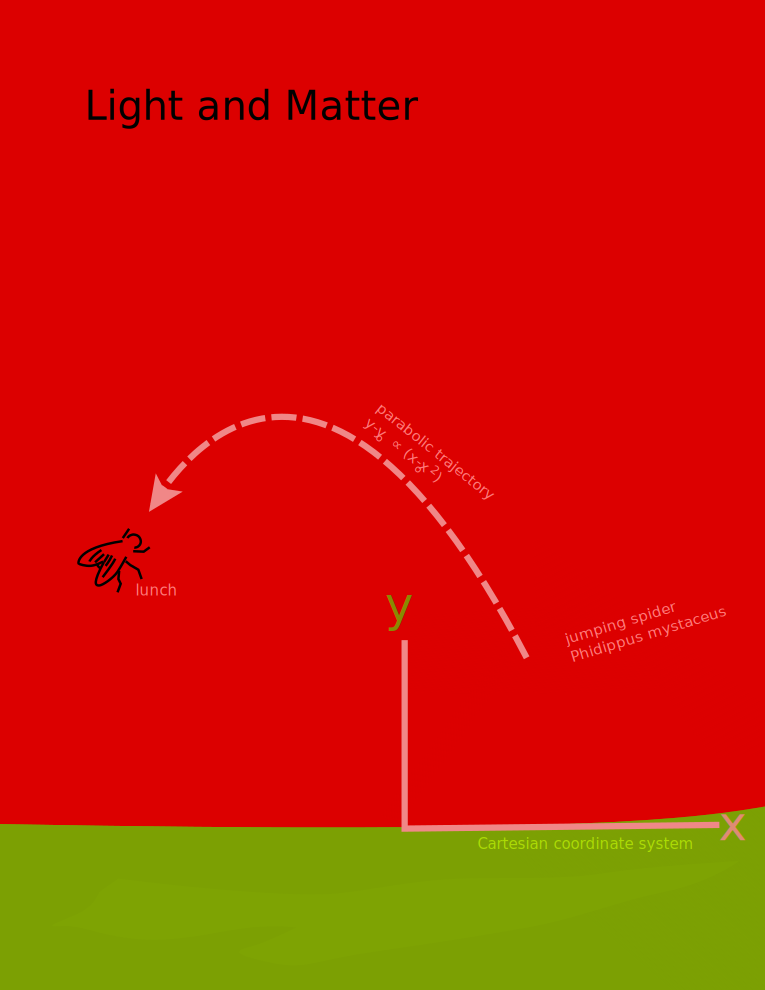
\includegraphics{\chapdir/figs/cover}\\
}
}%
\\

\pagebreak[4]

  \zerosizebox{-10mm}{140mm}{
    \noindent{}copyright 2006 Benjamin Crowell\vspace{10mm}
  }

  \zerosizebox{-10mm}{159mm}{
    rev. \today\vspace{10mm}
  }



  \zerosizebox{-10mm}{213mm}{
    \noindent{}\begin{minipage}{100mm}
    \noindent{}\begin{tabular}{p{9mm}p{95mm}}
    \zerosizebox{0mm}{14mm}{\anonymousinlinefig{cc-by-sa}} &
    This book is licensed under the 
Creative Commons
Attribution-ShareAlike license, version 3.0,
http://creativecommons.org/licenses/by-sa/3.0/,
    except for those photographs and
    drawings of which I am not the author, as listed in the photo credits.
    If you agree to the license, it grants you certain privileges that
    you would not otherwise have, such as the right to copy the book,
    or download the digital version free of charge from
    www.lightandmatter.com. At your option, you may also copy this book
    under the GNU Free Documentation License version 1.2, http://www.gnu.org/licenses/fdl.txt,
    with no invariant sections, no front-cover texts, and no back-cover texts.
    \end{tabular}
    \end{minipage}
}

\yesiwantarabic
\nomarginlayout
\vspace{10mm}\begin{center}\bfseries\sffamily{}\noindent{}{\huge Brief Contents}\end{center}\vspace{10mm}

\newcommand{\brieftocpartstyle}{\large\sffamily{}}
\newcommand{\brieftocchstyle}{\normalsize\sffamily{}}
\newcommand{\brieftocvert}{7mm}
\newcommand{\brieftochoriz}{\hspace{20mm}}
\newcommand{\brieftoctabularwidth}{90mm}

\noindent\brieftochoriz\brieftocchstyle\begin{tabular}{rp{\brieftoctabularwidth}}
\brieftocentry[\hfill]{ch:intro}{Introduction and review} \\
\brieftocentry[\hfill]{ch:scaling}{Scaling and estimation} \end{tabular}

\vspace{\brieftocvert}

\noindent\brieftochoriz\brieftocchstyle\begin{tabular}{rp{\brieftoctabularwidth}}

& \textit{\brieftocpartstyle Motion in one dimension}\\
\brieftocentry[\hfill]{ch:motion}{Velocity and relative motion} \\
\brieftocentry[\hfill]{ch:acceleration}{Acceleration and free fall} \\
\brieftocentry[\hfill]{ch:newton}{Force and motion} \\
\brieftocentry[\hfill]{ch:forces}{Analysis of forces} \end{tabular}

\vspace{\brieftocvert}

\noindent\brieftochoriz\brieftocchstyle\begin{tabular}{rp{\brieftoctabularwidth}}

& \textit{\brieftocpartstyle Motion in three dimensions}\\
\brieftocentry[\hfill]{ch:three-d}{Newton's laws in three dimensions} \\
\brieftocentry[\hfill]{ch:vectors}{Vectors} \\
\brieftocentry[\hfill]{ch:vectors-and-motion}{Vectors and motion} \\
\brieftocentry[\hfill]{ch:circular-motion}{Circular motion} \\
\brieftocentry[\hfill]{ch:gravity}{Gravity} \end{tabular}

\vspace{\brieftocvert}

\noindent\brieftochoriz\brieftocchstyle\begin{tabular}{rp{\brieftoctabularwidth}}

& \textit{\brieftocpartstyle Conservation laws}\\
\brieftocentry[\hfill]{ch:energy}{Conservation of energy} \\
\brieftocentry[\hfill]{ch:energy-zoo}{Simplifying the energy zoo} \\
\brieftocentry[\hfill]{ch:work}{Work: the transfer of mechanical energy} \\
\brieftocentry[\hfill]{ch:momentum}{Conservation of momentum} \\
\brieftocentry[\hfill]{ch:angular-momentum}{Conservation of  angular momentum} \\
\end{tabular}

\vspace{\brieftocvert}

\noindent\brieftochoriz\brieftocchstyle\begin{tabular}{rp{\brieftoctabularwidth}}

& \textit{\brieftocpartstyle Vibrations}\\
\brieftocentry[\hfill]{ch:vibrations}{Vibrations} \\
\brieftocentry[\hfill]{ch:resonance}{Resonance} 
\end{tabular}



\onecolumn\vfill
\mynormaltype

\pagebreak[4]

\vspace{0mm}
\begin{center}
\noindent\huge\bfseries\sffamily{}Contents\mynormaltype
\end{center}
\vspace{0mm}
\begin{multicols}{2}
  \tableofcontents
  \setcounter{unbalance}{0}
\end{multicols}
\normallayout\onecolumn

%========================= main matter =========================
\mainmatter
%-- I want the whole book numbered sequentially, arabic:
  \pagenumbering{arabic} 
  \addtocounter{page}{10}
\parafmt
\myeqnspacing % Do this early and often, since it gets reset by \normalsize
%========================= chapters =========================
\setcounter{chapter}{-1}
\wugga%used to be needed after preface
    \renewcommand{\chapdir}{pr}\include{pr/atemp}
    \renewcommand{\chapdir}{pr}\include{pr/btemp}
    \renewcommand{\chapdir}{n1}\include{n1/atemp}
    \renewcommand{\chapdir}{n1}\include{n1/btemp}
    \renewcommand{\chapdir}{n1}\include{n1/ctemp}
    \renewcommand{\chapdir}{n1}\include{n1/dtemp}
    \renewcommand{\chapdir}{n3}\include{n3/atemp}
    \renewcommand{\chapdir}{n3}\include{n3/btemp}
    \renewcommand{\chapdir}{n3}\include{n3/ctemp}
    \renewcommand{\chapdir}{n3}\include{n3/dtemp}
    \renewcommand{\chapdir}{n3}\include{n3/etemp}
    \renewcommand{\chapdir}{cl}\include{cl/atemp}
    \renewcommand{\chapdir}{cl}\include{cl/btemp}
    \renewcommand{\chapdir}{cl}\include{cl/ctemp}
    \renewcommand{\chapdir}{cl}\include{cl/dtemp}
    \renewcommand{\chapdir}{cl}\include{cl/etemp}
    \renewcommand{\chapdir}{vw}\include{vw/atemp}
	\formatchtoc{\large}{\quad\contentspage}{4mm} % This has to go before the last chapter.
        \addtocontents{toc}{\vspace{5mm}}% For reasons I don't understand, this actually comes *after* the final chapter.
    \renewcommand{\chapdir}{vw}\include{vw/btemp}
%
    \widelayout
    \renewcommand{\chapdir}{end}
    \include{end/skillstemp}
    \twocolumn\include{end/pythontemp}
    \onecolumn\include{end/hwanstemp}
    \onecolumn\include{end/photocreditstemp}
%========================= index =========================
\label{splits:index}\printindex
%========================= data tables, etc. =========================
        \blankchaptermarks\label{splits:data}
	\huge{\bfseries{\sffamily{Trig Table}}}\normalsize\normalfont

\begin{tabular}{rrrrrrrrrrrrrr}
$\theta$ & $\sin\theta$ & $\cos\theta$ & $\tan\theta$ & &
$\theta$ & $\sin\theta$ & $\cos\theta$ & $\tan\theta$ & &
$\theta$ & $\sin\theta$ & $\cos\theta$ & $\tan\theta$ \\
\cline{1-4}  \cline{6-9}  \cline{11-14}
$0\degunit$ &  0.000  &  1.000  &  0.000 & & $30\degunit$ &  0.500  &  0.866  &  0.577 & & $60\degunit$ &  0.866  &  0.500  &  1.732\\
$1\degunit$ &  0.017  &  1.000  &  0.017 & & $31\degunit$ &  0.515  &  0.857  &  0.601 & & $61\degunit$ &  0.875  &  0.485  &  1.804\\
$2\degunit$ &  0.035  &  0.999  &  0.035 & & $32\degunit$ &  0.530  &  0.848  &  0.625 & & $62\degunit$ &  0.883  &  0.469  &  1.881\\
$3\degunit$ &  0.052  &  0.999  &  0.052 & & $33\degunit$ &  0.545  &  0.839  &  0.649 & & $63\degunit$ &  0.891  &  0.454  &  1.963\\
$4\degunit$ &  0.070  &  0.998  &  0.070 & & $34\degunit$ &  0.559  &  0.829  &  0.675 & & $64\degunit$ &  0.899  &  0.438  &  2.050\\
$5\degunit$ &  0.087  &  0.996  &  0.087 & & $35\degunit$ &  0.574  &  0.819  &  0.700 & & $65\degunit$ &  0.906  &  0.423  &  2.145\\
$6\degunit$ &  0.105  &  0.995  &  0.105 & & $36\degunit$ &  0.588  &  0.809  &  0.727 & & $66\degunit$ &  0.914  &  0.407  &  2.246\\
$7\degunit$ &  0.122  &  0.993  &  0.123 & & $37\degunit$ &  0.602  &  0.799  &  0.754 & & $67\degunit$ &  0.921  &  0.391  &  2.356\\
$8\degunit$ &  0.139  &  0.990  &  0.141 & & $38\degunit$ &  0.616  &  0.788  &  0.781 & & $68\degunit$ &  0.927  &  0.375  &  2.475\\
$9\degunit$ &  0.156  &  0.988  &  0.158 & & $39\degunit$ &  0.629  &  0.777  &  0.810 & & $69\degunit$ &  0.934  &  0.358  &  2.605\\
$10\degunit$ &  0.174  &  0.985  &  0.176 & & $40\degunit$ &  0.643  &  0.766  &  0.839 & & $70\degunit$ &  0.940  &  0.342  &  2.747\\
$11\degunit$ &  0.191  &  0.982  &  0.194 & & $41\degunit$ &  0.656  &  0.755  &  0.869 & & $71\degunit$ &  0.946  &  0.326  &  2.904\\
$12\degunit$ &  0.208  &  0.978  &  0.213 & & $42\degunit$ &  0.669  &  0.743  &  0.900 & & $72\degunit$ &  0.951  &  0.309  &  3.078\\
$13\degunit$ &  0.225  &  0.974  &  0.231 & & $43\degunit$ &  0.682  &  0.731  &  0.933 & & $73\degunit$ &  0.956  &  0.292  &  3.271\\
$14\degunit$ &  0.242  &  0.970  &  0.249 & & $44\degunit$ &  0.695  &  0.719  &  0.966 & & $74\degunit$ &  0.961  &  0.276  &  3.487\\
$15\degunit$ &  0.259  &  0.966  &  0.268 & & $45\degunit$ &  0.707  &  0.707  &  1.000 & & $75\degunit$ &  0.966  &  0.259  &  3.732\\
$16\degunit$ &  0.276  &  0.961  &  0.287 & & $46\degunit$ &  0.719  &  0.695  &  1.036 & & $76\degunit$ &  0.970  &  0.242  &  4.011\\
$17\degunit$ &  0.292  &  0.956  &  0.306 & & $47\degunit$ &  0.731  &  0.682  &  1.072 & & $77\degunit$ &  0.974  &  0.225  &  4.331\\
$18\degunit$ &  0.309  &  0.951  &  0.325 & & $48\degunit$ &  0.743  &  0.669  &  1.111 & & $78\degunit$ &  0.978  &  0.208  &  4.705\\
$19\degunit$ &  0.326  &  0.946  &  0.344 & & $49\degunit$ &  0.755  &  0.656  &  1.150 & & $79\degunit$ &  0.982  &  0.191  &  5.145\\
$20\degunit$ &  0.342  &  0.940  &  0.364 & & $50\degunit$ &  0.766  &  0.643  &  1.192 & & $80\degunit$ &  0.985  &  0.174  &  5.671\\
$21\degunit$ &  0.358  &  0.934  &  0.384 & & $51\degunit$ &  0.777  &  0.629  &  1.235 & & $81\degunit$ &  0.988  &  0.156  &  6.314\\
$22\degunit$ &  0.375  &  0.927  &  0.404 & & $52\degunit$ &  0.788  &  0.616  &  1.280 & & $82\degunit$ &  0.990  &  0.139  &  7.115\\
$23\degunit$ &  0.391  &  0.921  &  0.424 & & $53\degunit$ &  0.799  &  0.602  &  1.327 & & $83\degunit$ &  0.993  &  0.122  &  8.144\\
$24\degunit$ &  0.407  &  0.914  &  0.445 & & $54\degunit$ &  0.809  &  0.588  &  1.376 & & $84\degunit$ &  0.995  &  0.105  &  9.514\\
$25\degunit$ &  0.423  &  0.906  &  0.466 & & $55\degunit$ &  0.819  &  0.574  &  1.428 & & $85\degunit$ &  0.996  &  0.087  & 11.430\\
$26\degunit$ &  0.438  &  0.899  &  0.488 & & $56\degunit$ &  0.829  &  0.559  &  1.483 & & $86\degunit$ &  0.998  &  0.070  & 14.301\\
$27\degunit$ &  0.454  &  0.891  &  0.510 & & $57\degunit$ &  0.839  &  0.545  &  1.540 & & $87\degunit$ &  0.999  &  0.052  & 19.081\\
$28\degunit$ &  0.469  &  0.883  &  0.532 & & $58\degunit$ &  0.848  &  0.530  &  1.600 & & $88\degunit$ &  0.999  &  0.035  & 28.636\\
$29\degunit$ &  0.485  &  0.875  &  0.554 & & $59\degunit$ &  0.857  &  0.515  &  1.664 & & $89\degunit$ &  1.000  &  0.017  & 57.290\\
&&&&& &&&&& $90\degunit$ &  1.000  &  0.000  & $\infty$\\
\end{tabular}
\pagebreak[4]
	\twocolumn[\begin{center}\huge{\bfseries{\sffamily{Mathematical Review}}}\end{center}]\normalsize\normalfont

\newcommand{\mathsummaryfont}{\normalsize\normalfont\small}
\newenvironment{ind}
	{%
	  	\setlength{\saveleftskip}{\leftskip}%
  		\addtolength{\leftskip}{10mm}%
                \noindent%
	}
	{%
		\par\setlength{\leftskip}{\saveleftskip} \par\myeqnspacing%
                \indentedcorrend%
	}
\newcommand{\hdr}[1]{\noindent\bfseries{\small\sffamily{#1}}\normalsize\mathsummaryfont}

\mathsummaryfont

\hdr{Algebra}

\noindent Quadratic equation:

\begin{ind}
  The solutions of $ax^2+bx+c=0$ \\
  are $x=\frac{-b\pm\sqrt{b^2-4ac}}{2a}$ \quad .
\end{ind}

\noindent Logarithms and exponentials:

\begin{ind}
  \begin{equation*}   \ln(ab)=\ln a + \ln b    \end{equation*}
  \begin{equation*}   e^{a+b} = e^ae^b    \end{equation*}
  \begin{equation*}   \ln e^x = e^{\ln x} = x    \end{equation*}
  \begin{equation*}   \ln(a^b) = b \ln a    \end{equation*}
\end{ind}

\hdr{Geometry, area, and volume}

\noindent\begin{tabular}{ll}
  area of a triangle of base $b$ and height $h$     & = $\frac{1}{2}bh$ \\
  circumference of a circle of radius $r$           &= $2\pi r$ \\
  area of a circle of radius $r$                    &= $\pi r^2$ \\
  surface area of a sphere of radius $r$            &= $4\pi r^2$ \\
  volume of a sphere of radius $r$                  &= $\frac{4}{3}\pi r^3$
\end{tabular}

\hdr{Trigonometry with a right triangle}

\noindent\anonymousinlinefig{trig}\\
  \begin{equation*}
 \sin\theta  = o/h \quad
 \cos\theta = a/h \quad
 \tan\theta = o/a
 \end{equation*}

Pythagorean theorem: $h^2=a^2+o^2$

\hdr{Trigonometry with any triangle}

\anonymousinlinefig{trig-any-triangle}\\
Law of Sines:
  \begin{equation*} \frac{\sin\alpha}{A}=\frac{\sin\beta}{B}=\frac{\sin\gamma}{C} \end{equation*}

\noindent Law of Cosines:
  \begin{equation*} C^2 = A^2 + B^2 - 2AB \cos \gamma \end{equation*}

%--------------------------------------------------------------

\pagebreak[4]

\hdr{Properties of the derivative and integral (for students in calculus-based
courses)}

\noindent Let $f$ and $g$ be functions of $x$, and let $c$ be a constant.

\noindent Linearity of the derivative:

\begin{equation*} \frac{\der}{\der x}(cf)=c \frac{\der f}{\der x} \end{equation*}

\begin{equation*} \frac{\der}{\der x}(f+g)=\frac{\der f}{\der x} + \frac{\der g}{\der x} \end{equation*}

\noindent The chain rule:

\begin{equation*} \frac{\der}{\der x}f(g(x)) = f'(g(x))g'(x) \end{equation*}

\noindent Derivatives of products and quotients:

\begin{equation*} \frac{\der}{\der x} (fg) = \frac{\der f}{\der x} g + \frac{\der g}{\der x} f\end{equation*}

\begin{equation*} \frac{\der}{\der x}\left(\frac{f}{g}\right) = \frac{f'}{g}-\frac{fg'}{g^2}\end{equation*}

\noindent Some derivatives:


\begin{tabular}{ll}
\multicolumn{2}{c}{$\frac{\der}{\der x} x^m = mx^{m-1},\ \text{except for $m=0$}$}\\
$\frac{\der}{\der x}\sin x = \cos x$ &
$\frac{\der}{\der x}\cos x = -\sin x$ \\
$\frac{\der}{\der x}e^x = e^x$ &
$\frac{\der}{\der x}\ln x = \frac{1}{x} $
\end{tabular}

\noindent Linearity of the integral:
\begin{equation*} \int cf(x)\der x = c\int f(x)\der x\end{equation*}
\begin{equation*} \int\left[f(x)+g(x)\right] = \int f(x) \der x + \int g(x) \der x \end{equation*}

\noindent The fundamental theorem of calculus:\\
The derivative and the integral undo each other, in the following sense:
\begin{equation*} \int_a^b f'(x)\der x = f(b)-f(a) \end{equation*}


\normalsize\normalfont
\pagebreak[4]
        \refstepcounter{appendixctr}\label{dataappendix}%
\appendix\chapter{Appendix \ref{dataappendix}: Useful Data}

\mysubsection[0]{Notation and terminology, compared with other books}\label{notationcompared}
Almost all the notation and terminology in \emph{Simple Nature} is standard, but there
are some cases where there is no universal standard, and a very few cases where
I've intentionally deviated from a universal standard. The notation used by physicists
is also different from that used by electrical and mechanical engineers; I use
physics terminology and notation (notably $\sqrt{-1}=i$, not $j$, and ``torque'' rather
than ``moment''), but employ the SI system of units used in engineering, rather than
the cgs units favored by some physicists.

\noindent Nonstandard terminology:
\begin{description}
	\item[Potential energy] is referred to in this book as \emph{interaction energy}, or
		according to its type: \emph{gravitational energy}, \emph{electrical energy}, etc.
	\item[The potential,] in an electrical context, is referred to as \emph{voltage},
		e.g. I say that $V=kq/r$ is the voltage surrounding a point charge.
	\item[Heat and thermal energy] are both referred to as \emph{heat}. This is in keeping
		with casual usage among scientists, but formal written usage dictates
		the use of ``thermal energy'' to mean the kinetic energy an object has because
		of its molecules' random motion, while ``heat'' is
		the transfer of thermal energy.
\end{description}

\noindent Notation for which there is no universal standard:
\begin{description}
	\item[Kinetic energy] is written $K$. Standard notation is $K$, $T$, or $KE$.
	\item[Interaction energy] is written $U$. Standard notation is $U$, $V$, or $PE$.
	\item[The unit vectors] are $\hat{\vc{x}},\hat{\vc{y}},\hat{\vc{z}}$. 
		Standard notation is either $\hat{\vc{x}},\hat{\vc{y}},\hat{\vc{z}}$ or
		$\hat{\vc{i}},\hat{\vc{j}},\hat{\vc{k}}$.
	\item[Distance from an axis] in cylindrical coordinates is $R$. A more common
		notation in math books is $\rho$, but this would conflict with the standard
		physics notation for the charge density.
	\item[Vibrations] do not have very well standardized terminology or notation. I use
		``frequency'' to refer to both $f$ and $\omega$, depending on the context to
		make it clear which is meant. The frequency of free, damped oscillations 
		is $\omega_f$, which is only approximately the same as $\omega_\zu{o}=\sqrt{k/m}$.
		The full width at half-maximum of the resonance peak (on a plot of energy versus
		frequency) is $\Delta\omega$.
	\item[The coupling constants] for electricity and magnetism are written as
		$k$ and $k/c^2$. This is standard notation, but it would be more common in 
		SI calculations to see everything expressed in terms of
		$\epsilon_\zu{o}=1/4\pi k$ and $\mu_\zu{o}=4\pi k/c^2$.
		Numerically, we have $k=8.99\times10^9\ \zu{N}\unitdot\zu{m}^2/\zu{C}^2$
		and $k/c^2=10^{-7}\ \zu{N}/\zu{A}^2$, the latter being
		an exact relation.
		
\end{description}
 %

\mysubsection[0]{Notation and units}\label{notationtable}
\noindent\begin{tabular}{|l|l|l|}
\hline
quantity	& unit	& symbol \\
\hline
distance	& meter, m	& $x, \Delta{}x$ \\
time	& second, s	& $t, \Delta{}t$ \\
mass	& kilogram, kg	& $m$ \\
density	& $\kgunit/\munit^3$	& $\rho$  \\
force	& newton, 1 N=$1\ \kgunit\unitdot\munit/\sunit^2$	& $F$ \\
velocity	& m/s	& $v$ \\
acceleration	& $\munit/\sunit^2$	& $a$ \\
gravitational field	& $\junit/\kgunit\unitdot\munit$ or $\munit/\sunit^2$	& $g$ \\
energy	& joule, J	& $E$ (also electric field)\\
momentum	& $\kgunit\unitdot\munit/\sunit$	& $p$ \\
angular momentum	& $\kgunit\unitdot\munit^2/\sunit$ or $\junit\unitdot\sunit$	& $L$ (also inductance)\\
power	& watt, 1 W = 1 J/s	& $P$ (also pressure) \\
pressure & 1 Pa=$1\ \nunit/\munit^2$	& $P$ (also power)\\
temperature	& K	& $T$ (also period)\\
period	& s	& $T$ (also temperature)\\
wavelength	& m	& $\lambda$ \\
frequency	& $\zu{s}^{-1}$ or Hz	& $f$ \\
charge	& coulomb, C	& $q$ \\
voltage	& volt, 1 V = 1 J/C	& $V$ \\
current	& ampere, 1 A = 1 C/s	& $I$ \\
resistance	& ohm, 1 $\Omega$ = 1 V/A	& $R$ \\
capacitance	& farad, 1 F = 1 C/V	& $C$ \\
inductance	& henry, 1 H = 1 $\zu{V}\unitdot\sunit/\zu{A}$	& $L$ (also angular momentum)\\
electric field	& V/m or N/C	& $E$ (also energy)\\
magnetic field	& tesla, 1 T = 1 $\nunit\unitdot\sunit/\zu{C}\unitdot\munit$	& $B$ \\
focal length	& m	& $f$ \\
magnification	& unitless	& $M$ \\
index of refraction	& unitless	& $n$ \\
electron wavefunction	& $\munit^{-3/2}$	& $\Psi$ \\
\hline
\end{tabular}
 %
\mysubsection[0]{Fundamental constants}
\noindent\begin{tabular}{|l|l|}
\hline
gravitational constant	& $G=6.67\times10^{-11}\ \junit\unitdot\munit/\kgunit^2$ \\
Boltzmann constant      & $k=1.38\times10^{-23}\ \junit/\kunit$\\
Coulomb constant	& $k=8.99\times10^9\ \junit\unitdot\munit/\zu{C}^2$ or $\nunit\unitdot\munit^2/\zu{C}^2$ \\
quantum of charge	& $e=1.60\times10^{-19}\ \zu{C}$ \\
speed of light	& $c=3.00\times10^8\ \zu{m/s}$ \\
Planck's constant	& $h=6.63\times10^{-34}\ \junit\unitdot\sunit$ \\
\hline
\end{tabular}\par
\noindent Note the use of the same notation, $k$, for both the Boltzmann constant and the Coulomb constant.


\mysubsection[0]{Metric prefixes}\label{metricprefixestable}\index{metric system!prefixes}
\noindent\begin{tabular}{|l|l|l|}
\hline
M-	& mega-			& $10^6$ \\
k-	& kilo-			& $10^3$ \\
m-	& milli-		& $10^{-3}$ \\
$\mu$- (Greek mu) & micro-	& $10^{-6}$ \\
n-	& nano-			& $10^{-9}$ \\
p-	& pico-			& $10^{-12}$ \\
f-	& femto-		& $10^{-15}$ \\
\hline
\end{tabular}

\noindent{}Note that the exponents go in steps of three.
The exception is centi-, $10^{-2}$, which is used only in the centimeter, and this
doesn't require memorization, because a cent is $10^{-2}$ dollars.
 %

\mysubsection[0]{Nonmetric units}\label{nonmetricunits}\index{units!nonmetric}
\noindent Nonmetric units in terms of metric ones:\\
\noindent\begin{tabular}{|l|l|}
\hline
1 inch	&= 25.4 mm (by definition)\\
1 pound (lb)	&= 4.5 newtons of force\\
1 scientific calorie &= 4.18 J\\
1 nutritional calorie &= $4.18\times10^3$ J\\
1 gallon &= $3.78\times10^3\ \zu{cm}^3$\\
1 horsepower &= 746 W\\
\hline
\end{tabular}

\noindent{}The pound is a unit of force, so it converts to newtons, not kilograms.
A one-kilogram mass at the earth's surface experiences a gravitational force of
$(1\ \kgunit)(9.8\ \munit/\sunit^2)=9.8\ \zu{N}=2.2\ \zu{lb}$. The nutritional
information on food packaging
typically gives energies in units of calories, but those so-called calories are
really kilocalories.

\noindent Relationships among U.S. units:\\
\noindent\begin{tabular}{|l|l|}
\hline
1 foot (ft)	&= 12 inches\\
1 yard (yd) &= 3 feet \\
1 mile (mi) &= 5280 feet\\
1 ounce (oz) &= 1/16 pound\\
\hline
\end{tabular}



\mysubsection[0]{The Greek alphabet}
\noindent\begin{tabular}{|lll|lll|lll|}
\hline
$\alpha$	& A			& alpha	& $\iota$		& I		& iota &  $\rho$	& P		& rho \\
$\beta$		& B			& beta	& $\kappa$	& K	& kappa & $\sigma$	& $\Sigma$	& sigma \\
$\gamma$	& $\Gamma$	& gamma	& $\lambda$ & $\Lambda$ & lambda & $\tau$ & T & tau\\
$\delta$	& $\Delta$		& delta	& $\mu$	& M	& mu & $\upsilon$ & Y & upsilon \\
$\epsilon$	& E			& epsilon	& $\nu$	& N		& nu & $\phi$ & $\Phi$ & phi\\
$\zeta$		& Z			& zeta	& $\xi$		& $\Xi$		& xi & $\chi$ & X & chi\\
$\eta$		& H			& eta	& o	& O		& omicron & $\psi$ & $\Psi$ & psi\\
$\theta$	& $\Theta$		& theta	& $\pi$		& $\Pi$		& pi & $\omega$ & $\Omega$ & omega\\
\hline
\end{tabular}
 %


\mysubsection[0]{Subatomic particles}\label{subatomicparticlesdata}
\noindent\begin{tabular}{|l|l|l|l|}
\hline
particle	& mass (kg)	& charge	& radius (fm) \\
\hline
electron	& $9.109\times10^{-31}$	& $-e$	& $\lesssim0.01$\\
proton	& $1.673\times10^{-27}$	& $+e$	& $\sim{}1.1$\\
neutron	& $1.675\times10^{-27}$	& 0		& $\sim{}1.1$\\
neutrino	& $\sim10^{-39}$ kg ?	& 0		& 	?\\
\hline
\end{tabular}

\noindent{}The radii of protons and neutrons can only be given
approximately, since they have fuzzy surfaces. For
comparison, a typical atom is about a million fm in radius.
 %




\mysubsection[0]{Earth, moon, and sun}
\noindent\begin{tabular}{|l|l|l|l|}
\hline
body		&	mass (kg)		&	radius (km)	&	radius of orbit (km) \\
\hline
earth	&	$5.97\times10^{24}$	&	$6.4\times10^{3}$	&	$1.49\times10^{8}$\\
moon	&	$7.35\times10^{22}$	&	$1.7\times10^{3}$	&	$3.84\times10^{5}$\\
sun		&	$1.99\times10^{30}$	&	$7.0\times10^{5}$	&	---\\
\hline
\end{tabular}
 %

\mysubsection[0]{The periodic table}
\anonymousinlinefig{periodictable}
 %

\mysubsection[0]{Atomic masses}
These atomic masses are given in atomic mass units (u), where by definition
the mass of an atom of the isotope carbon-12 equals 12 u. One atomic
mass unit is the same as about $1.66\times10^{-27}$ kg. Data are only
given for naturally occurring elements.

{\footnotesize
\begin{tabular}{|ll|ll|ll|ll|}
\hline
Ag	& 107.9	&Eu	& 152.0	&Mo	& 95.9	&Sc	& 45.0	\\
Al 	& 27.0 	&F	& 19.0	&N	& 14.0	&Se	& 79.0	\\
Ar 	& 39.9	&Fe	& 55.8	&Na	& 23.0	&Si	& 28.1	\\
As	& 74.9	&Ga	& 69.7	&Nb	& 92.9	&Sn	& 118.7	\\
Au	& 197.0	&Gd	& 157.2	&Nd	& 144.2	&Sr	& 87.6	\\
B	& 10.8	&Ge	& 72.6	&Ne	& 20.2	&Ta	& 180.9	\\
Ba	& 137.3	&H	& 1.0	&Ni	& 58.7	&Tb	& 158.9	\\
Be	& 9.0	&He	& 4.0	&O	& 16.0	&Te	& 127.6	\\
Bi	& 209.0	&Hf	& 178.5	&Os	& 190.2	&Ti	& 47.9	\\
Br	& 79.9	&Hg	& 200.6	&P	& 31.0	&Tl	& 204.4	\\
C	& 12.0	&Ho	& 164.9	&Pb	& 207.2	&Tm	& 168.9	\\
Ca	& 40.1	&In	& 114.8	&Pd	& 106.4	&U	& 238	\\
Ce	& 140.1	&Ir	& 192.2	&Pt	& 195.1	&V	& 50.9	\\
Cl	& 35.5	&K	& 39.1	&Pr	& 140.9	&W	& 183.8	\\
Co	& 58.9	&Kr	& 83.8	&Rb	& 85.5	&Xe	& 131.3	\\
Cr	& 52.0	&La	& 138.9	&Re	& 186.2	&Y	& 88.9	\\
Cs	& 132.9	&Li	& 6.9	&Rh	& 102.9	&Yb	& 173.0	\\
Cu	& 63.5	&Lu	& 175.0	&Ru	& 101.1	&Zn	& 65.4	\\
Dy	& 162.5	&Mg	& 24.3	&S	& 32.1	&Zr	& 91.2 	\\
Er	& 167.3	&Mn	& 54.9	&Sb 	& 121.8 	& & \\
\hline
\end{tabular}
}
 %

\end{document}
